\section{Behavioural reform costs}
\label{sec:behavioural}

The reforms of Section~\ref{sec:static} are costed \emph{statically}: each
schedule is re-applied to a fixed turnover distribution, and the revenue change is
the mechanical reclassification of firms with no response in turnover.
Section~\ref{sec:bunching} then shows that the bunching in my synthetic data is
mechanical, so a behavioural elasticity is not identified from it---the reduced-form
response is a placebo. Section~\ref{sec:model} supplies the one object that needs
no behavioural calibration at all: the exact, elasticity-free dominated region. What is
missing from this sequence is the behavioural layer itself---a costing that lets
firms re-optimise turnover when a reform changes the effective rate they face. This
section supplies that layer. I build an iso-elastic structural simulator that, for
an \emph{assumed} turnover elasticity $e$, re-solves each firm's optimum under a
counterfactual schedule and prices the resulting revenue effect. Because $e$ is not
identified from these data, I do not report a point estimate; I report an
$e$-sensitivity range. The simulator nests the static costing of
Section~\ref{sec:static} as its $e\to0$ limit, which I use below as a correctness
check rather than treat as a coincidence. This is honest infrastructure, and every
number in it is explicitly conditional on $e$.

\subsection{An iso-elastic structural simulator}
\label{ssec:simulator}

I adopt the iso-elastic firm problem of \citet{klevenwaseem2013}, in the
sufficient-statistics tradition of \citet{saez2010} and as applied to UK VAT by
\citet{liuetal2021}, but write it so that the tax falls on \emph{value added}
rather than on turnover. In this value-added statement---which I label
formulation~A---a firm of ability $n_i$ chooses turnover $y$ to maximise
\begin{equation}
  \pi_i(y) \;=\; (1-\delta_i)\,\bigl(1-\tau\,f(y)\bigr)\,y \;-\;
  C(y;n_i,e), \qquad
  C(y;n,e)=\frac{n}{1+1/e}\left(\frac{y}{n}\right)^{1+1/e},
  \label{eq:isoelastic}
\end{equation}
where $\delta_i\in[0,1)$ is the firm's \emph{deductible-input share} of turnover,
so that value added is $(1-\delta_i)\,y$; $\tau$ is the statutory VAT rate; and
$f(y)\in[0,1]$ is the fraction of $\tau$ that the schedule levies on the firm once
registered ($f=0$ below the threshold, $f=1$ for a fully registered firm under the
standard rate). Here $e>0$ is the elasticity of turnover with respect to the
net-of-tax rate.

It is essential to read $C$ correctly. Because the deductible inputs $\delta_i\,y$
are already netted out of revenue through the $(1-\delta_i)$ factor,
$C(y;n_i,e)$ must be understood as the firm's \emph{own-factor production
cost}---the labour and capital effort the firm itself supplies---and \emph{not} its
total cost of production. Reading $C$ as total cost would double-count the bought-in
inputs, which the value-added factor has already removed. Marginal own-factor cost
is $(y/n)^{1/e}$, so the undistorted optimum is $y=n$: ability $n$ is the firm's
frictionless turnover. A firm registered under a flat rate ($f\equiv1$) chooses
\begin{equation}
  y^{*} \;=\; n\,\bigl[(1-\delta)(1-\tau)\bigr]^{e},
  \label{eq:flat-optimum}
\end{equation}
so the retained wedge facing the firm is the product $(1-\delta)(1-\tau)$ of the
value-added share and the statutory net-of-tax rate, and one verifies directly
from~\eqref{eq:flat-optimum} that
$\mathrm{d}\ln y^{*}/\mathrm{d}\ln\!\bigl[(1-\delta)(1-\tau)\bigr]=e$, so $e$ is
exactly the knob that governs the intensive response.
Figure~\ref{fig:formulation_a_optima} traces the formulation-A profit and its
optima across the notch and taper schedules for three deductible shares, showing
how both the value-added optimum and the notch geometry shift with $\delta$: the
$(1-\delta)$ factor scales the whole curve down, and a higher $\delta$ pulls the
registered optimum back toward the threshold, eventually tipping the global
choice from the registered interior optimum to bunching at the notch.

\begin{figure}[htbp]
\centering
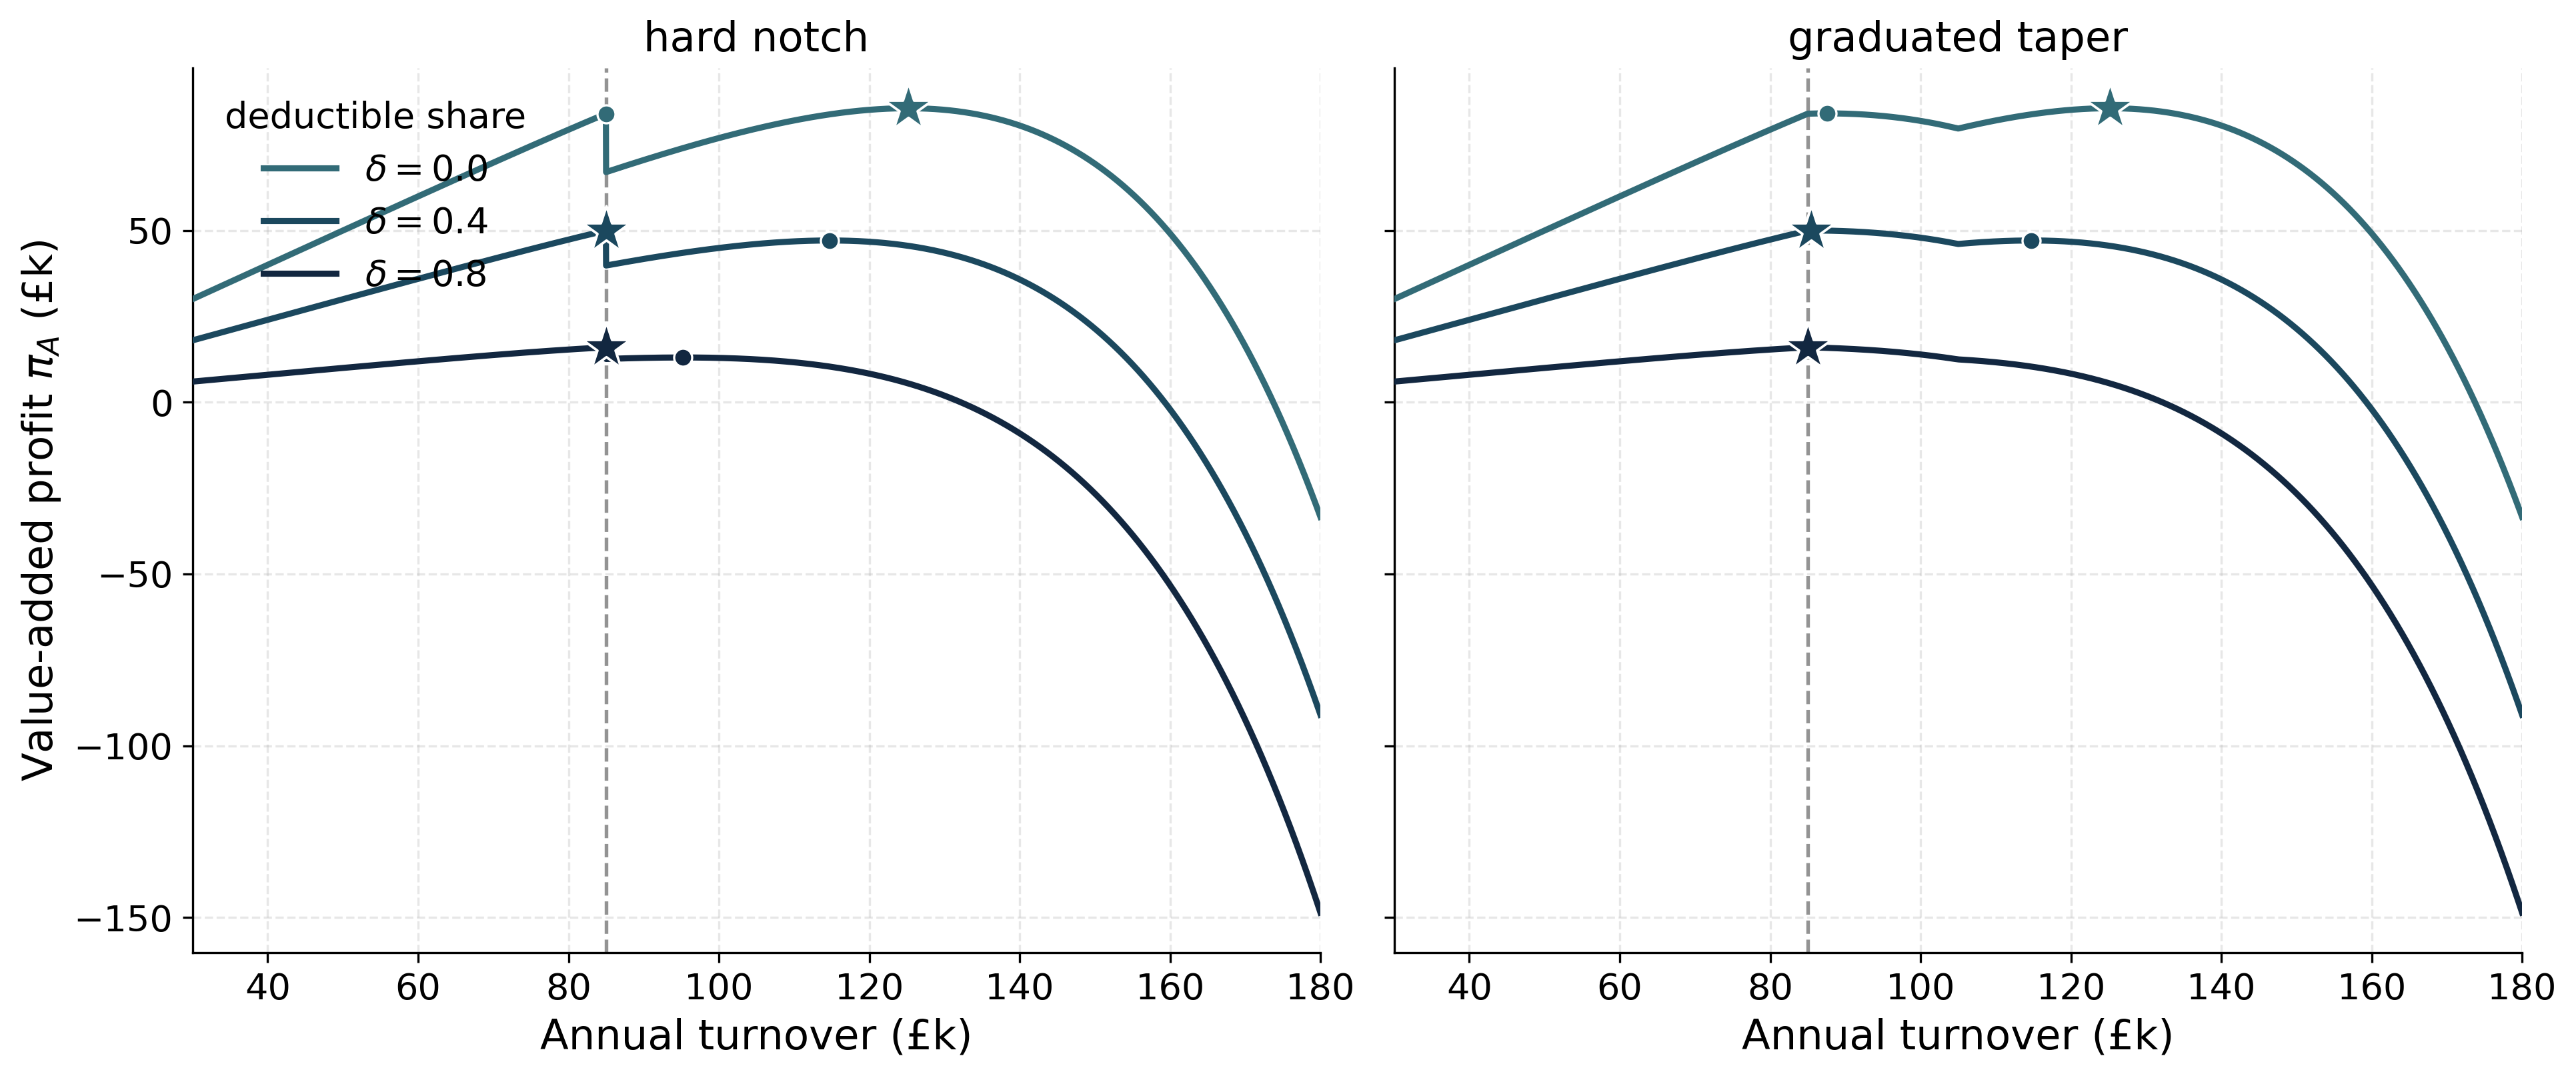
\includegraphics[width=0.85\textwidth]{figures/formulation_a_optima.png}
\caption{Optima of the value-added (formulation~A) profit
function~\eqref{eq:isoelastic}, $\pi_A(y)=(1-\delta)(1-\tau f(y))\,y-C(y;n,e)$,
at statutory rate $\tau=0.20$, ability $n=\pounds130$k and elasticity $e=0.17$,
under the hard registration notch (left) and the graduated
taper (right). Each panel overlays three deductible-input shares
$\delta\in\{0.0,0.4,0.8\}$; dots mark each curve's local maxima and the star its
global optimum, and the dashed vertical line is the \pounds85{,}000 threshold.
The value-added factor $(1-\delta)$ scales the whole curve down without moving
the frictionless optimum, while a higher $\delta$ shrinks the retained wedge
$(1-\delta)(1-\tau)$ and so pulls the registered optimum
$y^{*}=n[(1-\delta)(1-\tau)]^{e}$ back toward the threshold---eventually tipping
the global optimum from the registered interior peak to bunching at the notch,
consistent with the formulation-A discussion above.}
\label{fig:formulation_a_optima}
\end{figure}

\paragraph{Ability recovery.} To populate the simulator I recover an ability $n$
for each firm from its observed turnover under the baseline \pounds85{,}000 notch.
Given $e$, I set $n=y_{\mathrm{obs}}$ for an unregistered firm
($y_{\mathrm{obs}}<T^{*}$) and invert the registered-firm optimum for the rest.
Operationally I drive both the recovery and the forward solve off each firm's
calibrated \emph{net VAT rate} $\tau_i$---net remittance over turnover, that is
output VAT less input credits, which averages about $3\%$ of turnover in the
calibrated population (Section~\ref{sec:data})---so that
$n=y_{\mathrm{obs}}/(1-\tau_i)^{e}$ and the effective wedge is pinned to the firm's
calibrated net-VAT position rather than to the full statutory product
$(1-\delta_i)(1-\tau)$. The net rate $\tau_i$ is the firm's own remittance, and
\emph{not} the statutory $20\%$. This distinction is material: VAT is levied on
value added, not on turnover, so a firm remitting $3\%$ of its turnover has been
distorted as if it faced a net-of-tax rate near $0.97$, not $0.80$. Inverting at
the statutory $20\%$ would inflate the recovered ability gap, and hence every
counterfactual response, several-fold.

Formulation~A in~\eqref{eq:isoelastic} is the conceptual value-added statement of
exactly this tax, and the two representations coincide at $\delta=0$, where the
net-VAT wedge and the statutory net-of-tax rate agree. I do not, however, run the
recovery off the literal formulation-A wedge, and one caveat explains why. The
literal recovery $n=y_{\mathrm{obs}}/\bigl[(1-\delta_i)(1-\tau)\bigr]^{e}$ is
numerically fragile for firms with very high deductible shares: as $\delta_i\to1$
the retained wedge $(1-\delta_i)(1-\tau)\to0$ and the recovered ability diverges,
which would hand a handful of input-heavy firms an implausible weight in the
aggregate. Driving the costing off the calibrated net-VAT wedge $\tau_i$ sidesteps
this instability while pricing the same value-added tax. At present $\delta_i$ is
parametric---held at a calibrated value rather than measured firm by firm---and
grounding it in ONS Supply--Use and Annual Business Survey
value-added-to-turnover data is left to future work.

\paragraph{Forward solve.} Holding the recovered abilities $\{n_i\}$ and the
assumed $e$ fixed, I re-solve each firm's optimum under the reform schedule---the
raised threshold, the graduated taper, or the reduced-rate band---and aggregate the
resulting liabilities. The behavioural revenue effect is the difference between this
aggregate and the baseline. Because a reform that lowers the effective rate on the
band raises each affected firm's net-of-tax rate, the firm scales turnover up
toward its frictionless optimum,
\begin{equation}
  y^{*}_i \;=\; y_{\mathrm{obs},i}\,
  \left(\frac{1-\tau_{\mathrm{reform}}}{1-\tau_{\mathrm{base}}}\right)^{e}
  \;>\; y_{\mathrm{obs},i},
  \label{eq:rescale}
\end{equation}
so the taxed base broadens and partly offsets the static loss.

\paragraph{Conditional on $e$.} I am explicit about what this exercise is and is
not. Treating each firm's observed (mechanically calibrated) turnover as optimal
and inverting it for $n$ is an \emph{accounting anchor}, not structural
identification: it reproduces the baseline by construction but borrows no
information about the response. The elasticity $e$ is not identified from these data
(the placebo of Section~\ref{sec:bunching}), so every behavioural magnitude below is
conditional on the assumed $e$. The robust, $e$-free headline objects remain the
static cost of Section~\ref{sec:static} and the exact dominated region of
Section~\ref{sec:model}; this section's numbers are a disciplined sensitivity range,
not point estimates. The margin priced here is purely \emph{intensive}---firms scale
turnover as the effective rate moves. The extensive notch distortion, the discrete
incentive to suppress turnover and bunch below the threshold, is the separate
analytic object of Section~\ref{sec:model}; a reader should not expect re-bunching
dynamics here.

\subsection{Results}
\label{ssec:behavioural-results}

I sweep $e\in\{0.05,\,0.17,\,0.32\}$ and report the full sweep, treating
$e=0.17$ as an illustrative midpoint rather than a headline estimate. The low
value $0.05$ is of the order reported by \citet{klevenwaseem2013}; $0.32$ is the
mean implied by mapping the marginal-buncher condition through my notch; $0.17$ is
the median of that mapping. (These per-firm-mapping summaries are a different object
from the single aggregate marginal-buncher elasticity $\approx0.66$ tabulated in
Appendix~\ref{app:inference}, and differ from it numerically; both are mechanical,
non-identified artefacts of the calibration.) I flag the provenance plainly: the $0.17$ and $0.32$
values are read off the marginal-buncher condition applied to my notch geometry,
which inherits the mechanical bunching that Section~\ref{sec:bunching} shows to be
non-behavioural, so they are model-implied, not data-identified; the range's only
externally-anchored point is its lower end (the \citet{klevenwaseem2013} value of
$\approx 0.05$). I use them only to delimit a plausible sweep, and a reader
preferring a fully external range---for instance \citet{liuetal2021}'s UK VAT-base
elasticity---may substitute literature values for $e$ directly without changing the
conditional structure of the costing. The same mapping pins the marginal buncher
$n_H(e)$---the highest ability that still finds it optimal to bunch at the
threshold---at \pounds112{,}795 for $e=0.05$ (a frictionless excess
$\Delta y_{H}\equiv n_H-T^{*}\approx\pounds27.8$k, distinct from the empirical
bunching span $\Delta y^{*}=\pounds5.6$k of Appendix~\ref{app:inference}),
\pounds127{,}382 for $e=0.17$
($\approx\pounds42.4$k), and \pounds143{,}527 for $e=0.32$ ($\approx\pounds58.5$k),
consistent with the analytic dominated-region width $a=\pounds21{,}250$ of
Section~\ref{sec:model}.

Table~\ref{tab:behavioural_costs} reports the behavioural cost of each of the three
flat-rate reforms---the raised threshold and the two reduced-rate bands---measured
as the change in revenue relative to the \pounds85{,}000-notch baseline, alongside
the static figure of Table~\ref{tab:schedule_costs}, for each $e$. The direction is
uniform across these three: a larger $e$ makes each of them \emph{cheaper} in
revenue terms. The mechanism is~\eqref{eq:rescale}: each reform lowers the effective
rate on the band by a \emph{constant} amount, so firms scale turnover up toward
their frictionless optimum, broadening the taxed base and partly offsetting the
static loss. The offset is substantial: at $e=0.17$ the raised threshold costs
\(-\)\pounds292m against a static \(-\)\pounds508m, and the $10\%$ and $15\%$ bands
cost \(-\)\pounds273m and \(-\)\pounds135m against static \(-\)\pounds343m and
\(-\)\pounds171m. At the illustrative midpoint $e=0.17$, the number of firms re-optimising is
$50{,}155$ under the raised threshold, $61{,}187$ under the $10\%$ reduced rate, and
$51{,}226$ under the $15\%$ reduced rate. Figure~\ref{fig:reform_dist} traces these
costs across the full range of $e$, with each curve nesting onto its static value as
$e\to0$.

\paragraph{Why the graduated taper is excluded.} I do not report a behavioural cost
for the graduated taper, and I want to be candid about why. The taper carries two
behavioural channels that pull in opposite directions. The first is the
base-broadening channel shared with the flat reforms: as the \emph{average} rate a
firm faces falls, the firm scales its turnover up, which is cheaper for revenue in
exactly the way~\eqref{eq:rescale} captures. The second is a marginal-rate
distortion that is the taper's signature: because the taper's rate \emph{rises} with
turnover, raising output lifts the rate on \emph{all} of a firm's turnover, so the
firm faces an incentive to hold turnover down---a force that is costlier for
revenue, not cheaper. The iso-elastic cost used here can price the first, upward
channel but not the second, downward one. Imposing the full marginal-rate wedge in a
correct first-order-condition solve makes firms collapse to the band floor and yields
economically pathological revenue losses of the order of several billion pounds---an
artefact of a cost function that cannot represent the downward, marginal-rate-driven
response a taper induces, not a credible policy estimate. The net behavioural sign of
the taper is therefore ambiguous and not identified in this framework. I take this as
an honest scope limit, consistent with the paper's careful identification stance, and
report only the taper's robust, $e$-free objects---its static cost
(Section~\ref{sec:static}) and its exact, analytic removal of the dominated region
(Section~\ref{sec:model}).

\begin{table}[htbp]
\centering
\caption{Behavioural revenue effect of the three flat-rate reforms relative to the
\pounds85{,}000-notch baseline, by assumed turnover elasticity $e$, with the static
($e\to0$ limit) figure for comparison. Each behavioural figure re-solves every
firm's iso-elastic optimum~\eqref{eq:isoelastic} under the reform schedule, holding
recovered abilities and $e$ fixed. The final column reports the number of firms that
re-optimise at the illustrative midpoint $e=0.17$. Every behavioural figure is conditional on the
assumed, non-identified $e$. The graduated taper is excluded from the behavioural
costing; see the note below the table and the discussion that follows.}
\label{tab:behavioural_costs}
\begin{tabular}{lrrrrr}
\hline
Reform & Static & $e=0.05$ & $e=0.17$ & $e=0.32$ & Firms ($e{=}0.17$) \\
\hline
Raise threshold to \pounds100{,}000
  & $-\pounds508$m & $-\pounds444$m & $-\pounds292$m & $-\pounds111$m & $50{,}155$ \\
Reduced rate $10\%$ $[\pounds85\text{k},\pounds105\text{k}]$
  & $-\pounds343$m & $-\pounds322$m & $-\pounds273$m & $-\pounds210$m & $61{,}187$ \\
Reduced rate $15\%$ $[\pounds85\text{k},\pounds105\text{k}]$
  & $-\pounds171$m & $-\pounds160$m & $-\pounds135$m & $-\pounds107$m & $51{,}226$ \\
\hline
\end{tabular}

\smallskip
{\footnotesize \emph{Note.} The graduated taper is deliberately omitted from this
table. Its behavioural response cannot be credibly priced in the iso-elastic
framework, for the reason set out in the paragraph below; its robust, $e$-free
figures---the static cost of \(-\)\pounds336m and the exact removal of the dominated
region---are reported in Sections~\ref{sec:static} and~\ref{sec:model} instead.}
\end{table}

\paragraph{Validation: the $e\to0$ limit.} For the three flat-rate reforms the
simulator should reproduce the static costing as the response vanishes, and it does.
Taking $e\to0$ in the forward solve returns \(-\)\pounds507m for the raised
threshold, \(-\)\pounds343m for the $10\%$ reduced rate, and \(-\)\pounds171m for the
$15\%$ reduced rate---matching the static \(-\)\pounds508m, \(-\)\pounds343m, and
\(-\)\pounds171m of Table~\ref{tab:schedule_costs} to within about \pounds1m.
This is the intended nesting: when no firm responds, the behavioural cost collapses
to the mechanical reclassification effect, so the static costing is the $e=0$ corner
of the same machine, not a separate calculation. The nesting notably does \emph{not}
hold for the graduated taper---a further symptom that the iso-elastic cost cannot
represent the taper's marginal-rate channel, and an additional reason its behavioural
cost is not reported. I separately confirm numerically that
$\mathrm{d}\ln y^{*}/\mathrm{d}\ln(1-\tau)=e$ holds exactly in the solved population
for the flat reforms, so $e$ is indeed the governing knob.

\begin{figure}[htbp]
\centering
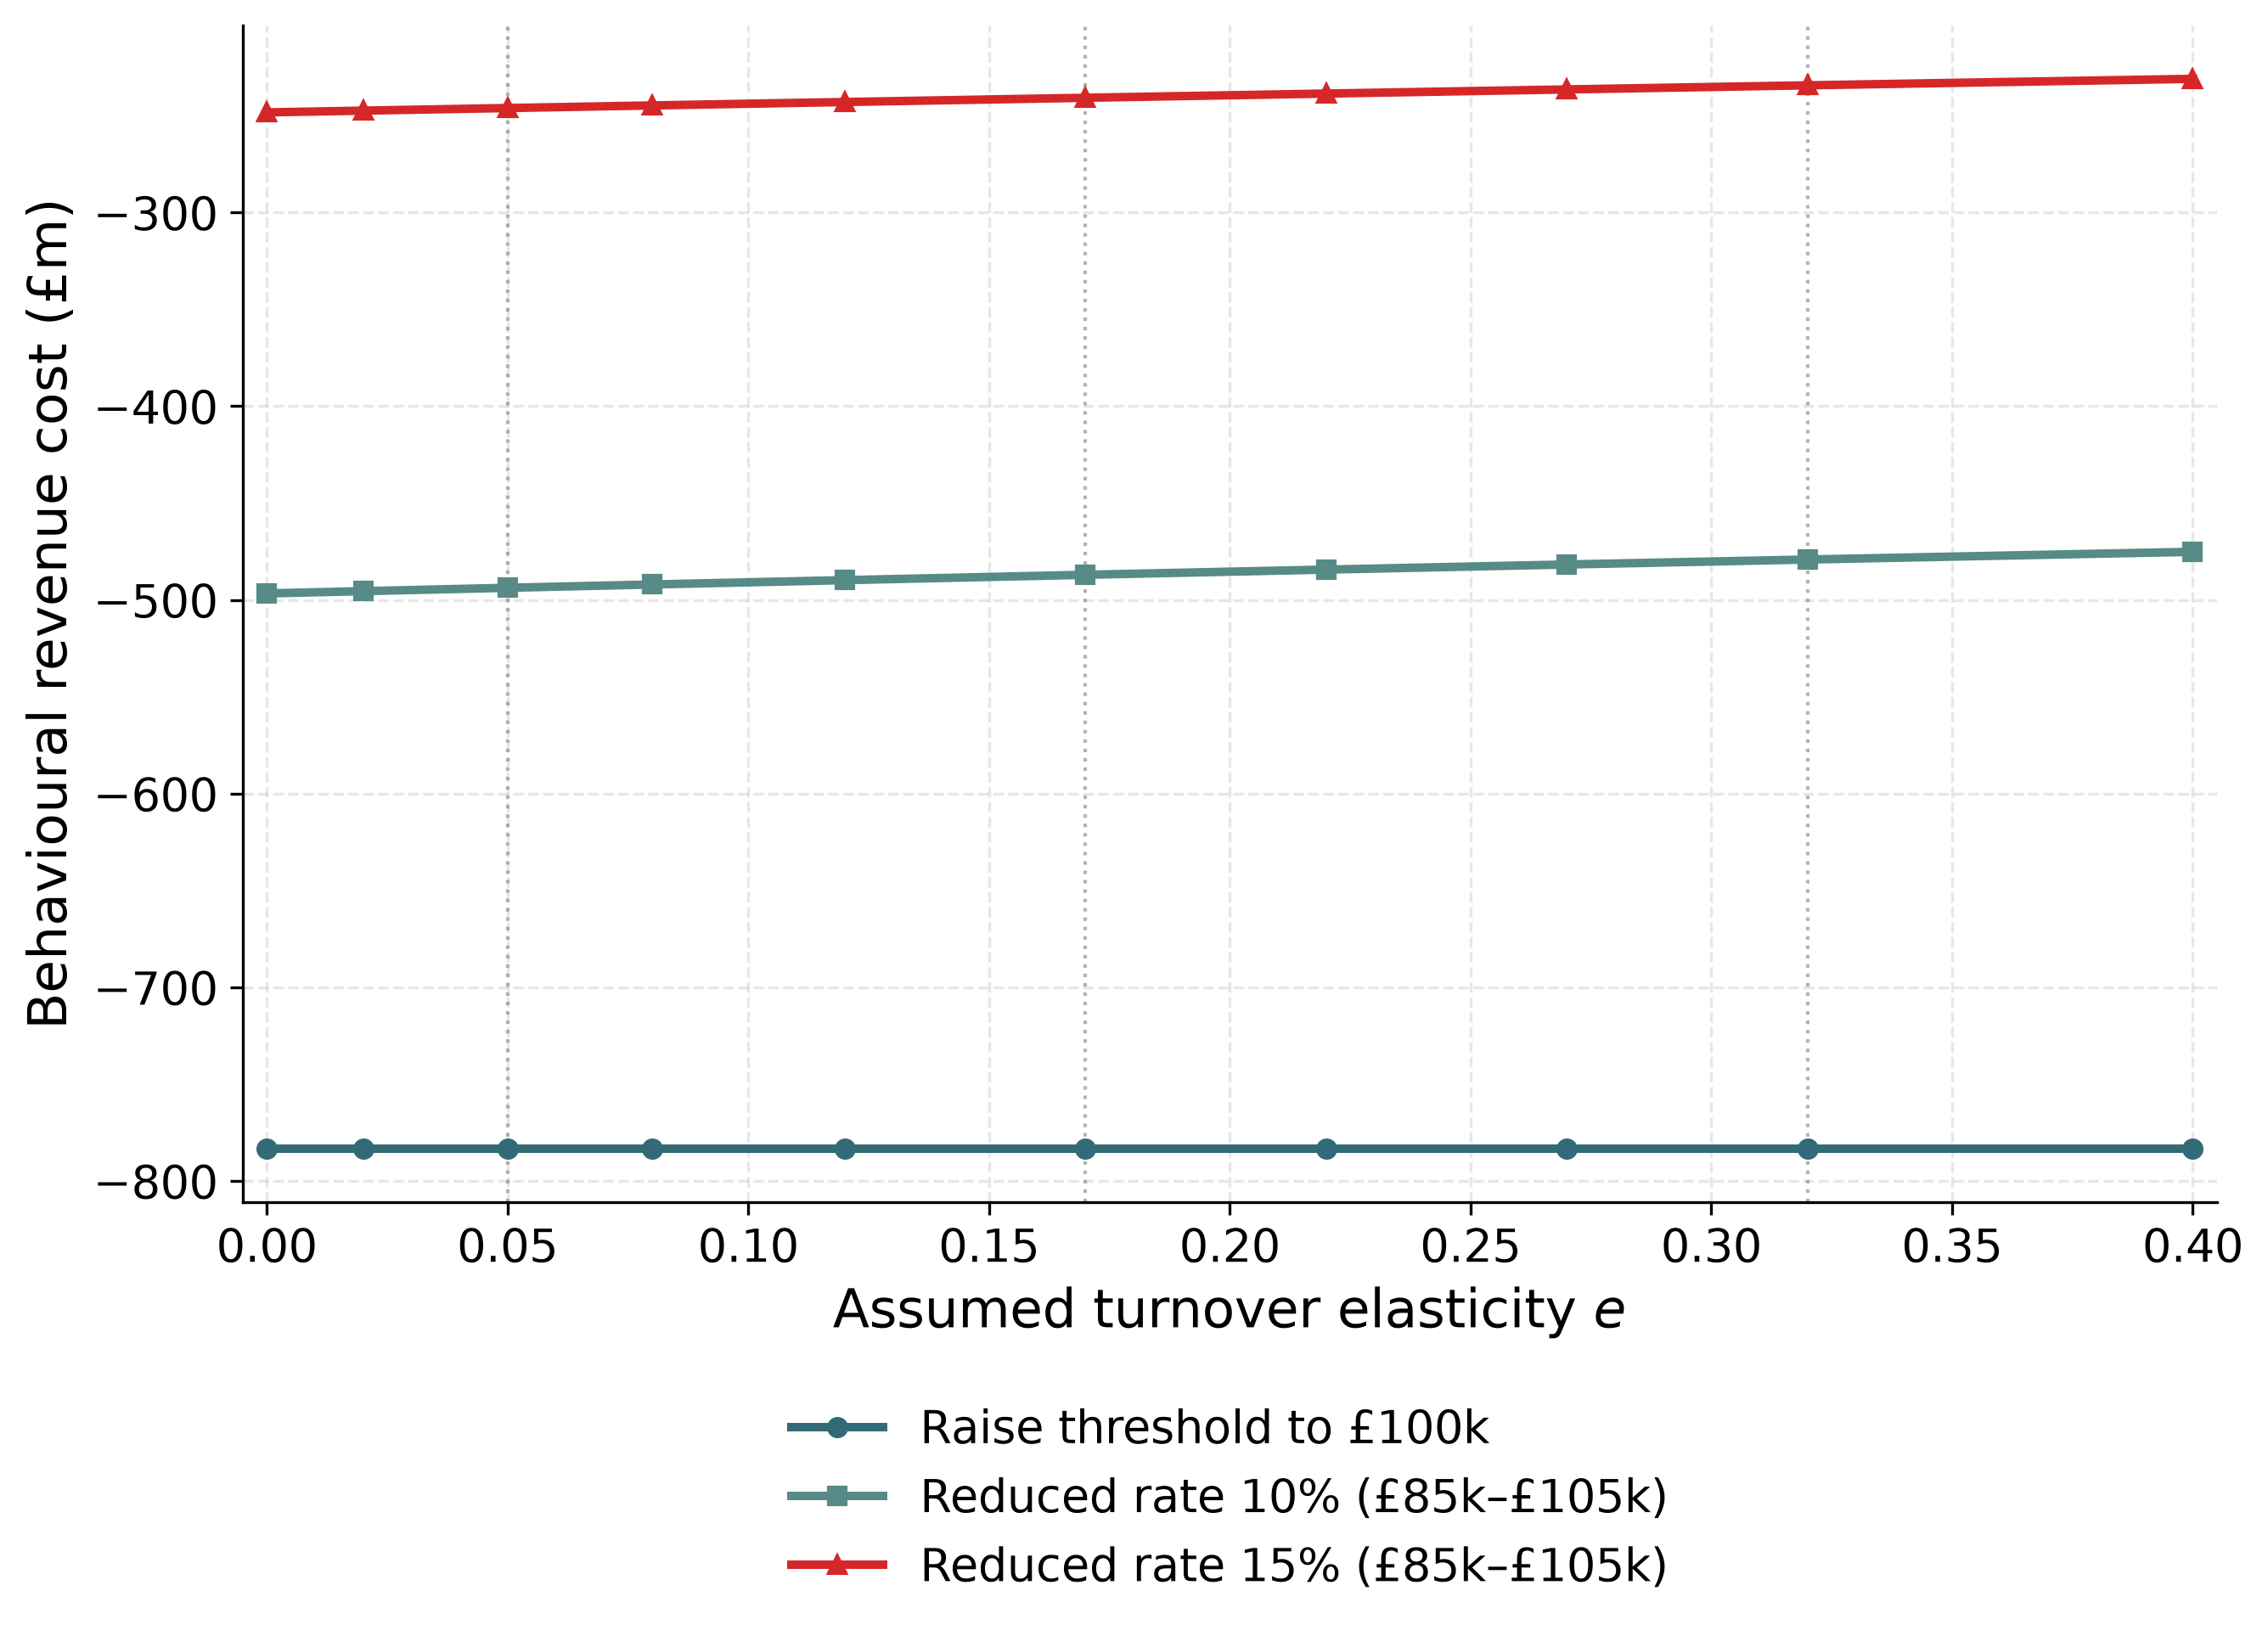
\includegraphics[width=0.78\textwidth]{figures/dynamic_cost_vs_elasticity.png}
\caption{Behavioural reform cost against the assumed turnover elasticity $e$, for
the three flat-rate reforms. Each curve is the change in revenue relative to the
\pounds85{,}000-notch baseline as $e$ varies; the intercept at $e=0$ is the static
cost of Table~\ref{tab:schedule_costs}, onto which the behavioural cost nests as the
response vanishes. As $e$ rises, firms scale turnover up toward their frictionless
optimum~\eqref{eq:rescale}, broadening the taxed base and making each reform cheaper.
The dotted lines mark the swept values $e\in\{0.05,0.17,0.32\}$ of
Table~\ref{tab:behavioural_costs}. The graduated taper is omitted: its behavioural
response is not credibly identified in this framework (see above). All magnitudes are
conditional on the assumed, non-identified $e$.}
\label{fig:reform_dist}
\end{figure}

This section completes the costing framework. Where Section~\ref{sec:static} prices
each reform mechanically and Section~\ref{sec:model} measures the distortion it
removes, the simulator here prices the \emph{level and rate} reforms
\emph{behaviourally}: it lets firms re-optimise turnover as the effective rate
changes and implies that, for any assumed $e$, the base-broadening response would
offset a fraction of the static revenue loss. The layer is bounded by what it can
and cannot identify. The behavioural magnitudes are conditional on an assumed,
non-identified $e$, and so are a sensitivity range rather than forecasts; and the
priced margin is purely \emph{intensive}, since the model re-scales turnover while
holding the extensive bunching response fixed. Crucially, the graduated taper's
behavioural response is \emph{not} credibly identified in this framework: its
base-broadening and marginal-rate channels pull in opposite directions and the
iso-elastic cost cannot net them, so I price it only statically and through its exact
dominated-region removal. The robust anchors of the paper therefore remain the
$e$-free static cost of Section~\ref{sec:static} and the exact dominated region of
Section~\ref{sec:model}; the contribution here is a disciplined, transparent layer
that prices the intensive behavioural response to the level and rate reforms once one
is willing to name an elasticity.
